\section{Условие лабораторной}

Моделируем информационный центр. В информационный центр приходят клиенты (пользователи) через интервал времени 10 ± 2 минуты. Если все три имеющихся оператора заняты, клиенту отказывают в обслуживании.
Операторы имеют разную производительность и могут обеспечивать обслуживание среднего запроса от пользователя за 20 ± 5, 40 ± 10 и 40 ± 20 ед. времени (минут).
Клиенты стараются занять свободного оператора с максимальной производительностью.
Полученные запросы сдаются в накопитель, откуда выбираются на обработку.
На первый компьютер — от первого и второго операторов, на второй --- от третьего.
Время обработки запроса в компьютерах — 15 и 30 минут соответственно.
Смоделировать процесс обработки 300 запросов. Определить вероятность отказа.

\section{Теоретическая часть}

\subsection{Схемы модели}

На рисунке \ref{img:blockDiagram} представлена структурная схема модели.

\begin{figure}[ht!]
	\centering
	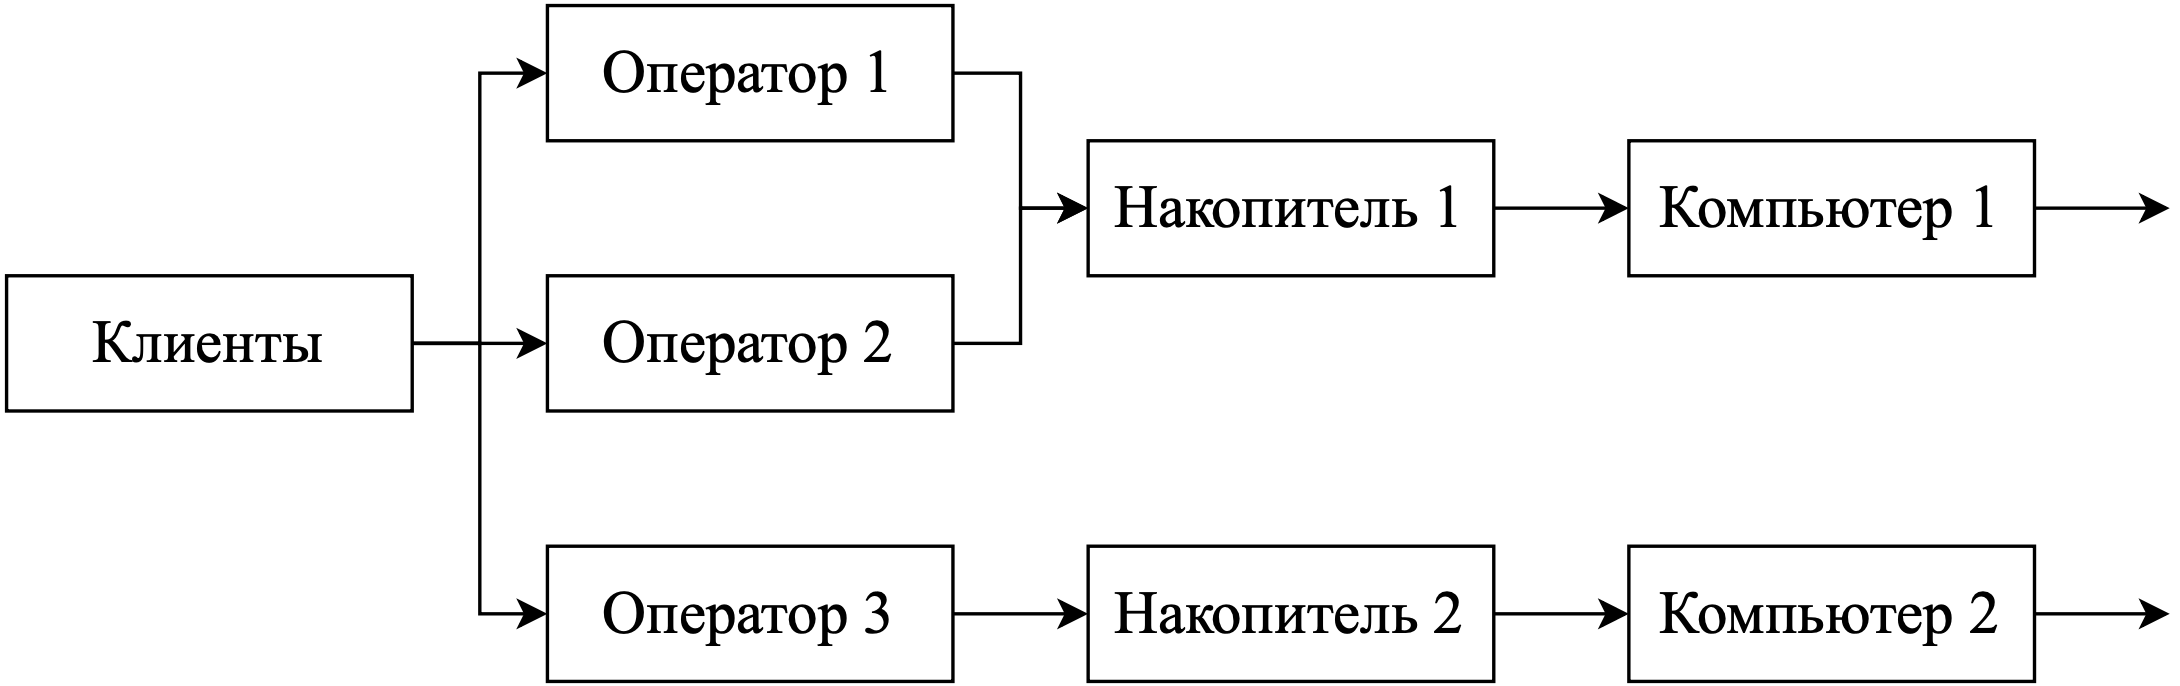
\includegraphics[width=0.6\linewidth]{../img/blockDiagram.png}
	\caption{Структурная схема модели}
	\label{img:blockDiagram}
\end{figure}

В процессе взаимодействия клиентов с информационным центром возможно два режима работы:

\begin{itemize}
	\item режим нормального обслуживания, когда клиент выбирает одного из свободных операторов, отдавая предпочтение тому, у кого максимальная производительность;
	\item режим отказа клиенту в обслуживании, когда все операторы заняты.
\end{itemize}

На рисунке \ref{img:queuingSystems} представлена схема модели в терминах систем массового обслуживания (СМО).

\begin{figure}[ht!]
	\centering
	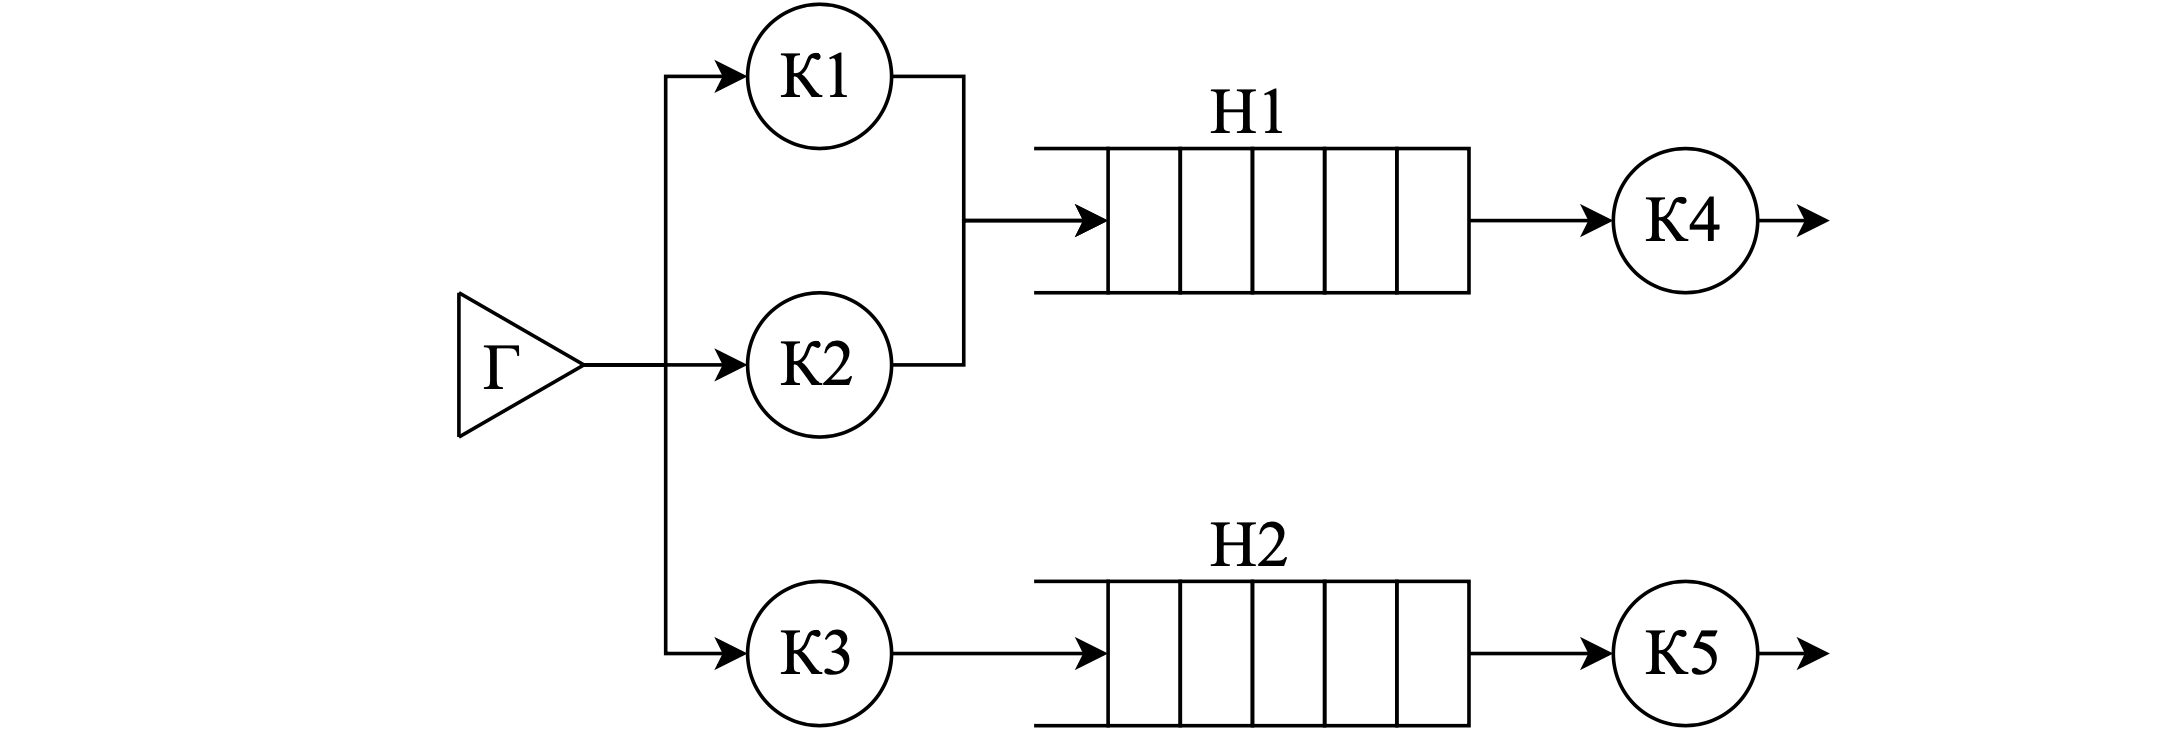
\includegraphics[width=0.6\linewidth]{../img/queuingSystems.png}
	\caption{Схема модели в терминах СМО}
	\label{img:queuingSystems}
\end{figure}

\subsection {Равномерное распределение}

Случайная величина $X$ имеет \textit{равномерное распределение} на отрезке~$[a,~b]$, если ее плотность распределения~$f(x)$ равна:
\begin{equation}
	p(x) =
	\begin{cases}
		\displaystyle\frac{1}{b - a}, & \quad \text{если } a \leq x \leq b;\\
		0,  & \quad \text{иначе}.
	\end{cases}
\end{equation}

При этом функция распределения~$F(x)$ равна:

\begin{equation}
	F(x) =
	\begin{cases}
		0,  & \quad x < a;\\
		\displaystyle\frac{x - a}{b - a}, & \quad a \leq x \leq b;\\
		1,  & \quad x > b.
	\end{cases}
\end{equation}

Обозначение: $X \sim R[a, b]$.

\begin{equation}
	T_{i} = a + (b - a) \cdot R,
\end{equation}

\noindent где $R$ --- псевдослучайное число от 0 до 1.

\subsection{Переменные и уравнение имитационной модели}

\textbf{Эндогенные переменные:}

\begin{itemize}
	\item время обработки задания $i$-ым оператором;
	\item время решения задания на $j$-ом компьютере.
\end{itemize}

\textbf{Экзогенные переменные:}

\begin{itemize}
	\item $n0$ — число обслуженных клиентов;
	\item $n1$ — число клиентов, получивших отказ.
\end{itemize}

Вероятность отказа в обслуживании клиента будет вычисляться как:

\begin{equation}
	P = \frac{n_0}{n_0 + n_1}
\end{equation}

\subsection{GPSS}

Язык GPSS – общецелевая система моделирования.

Транзакты представляют собой описание динамических процессов в
реальных системах. Они могут описывать как реальные физические объекты,
так и нефизические, например, канальная программа. Транзакты можно
генерировать и уничтожать в процессе моделирования. Основным атрибутом
любого транзакта является число параметров (от 0 до 1020).

Динамическими объектами являются транзакты, которые представляют собой единицы исследуемых потоков и производят ряд определённых
действий, продвигаясь по фиксированной структуре, представляющей собой
совокупность объектов других категорий.

Операционный объект. Блоки задают логику функционирования
системы и определяют маршрут движения транзактов между объектами
аппаратной категории. Это абстрактные элементы, на которые может быть
декомпозирована структура реальной системы. Воздействуя на эти объекты,
транзакты могут изменять их состояния и оказывать влияние на движение
других объектов.

Вычислительный объект. Служит для описания таких операций
в процессе моделирования, когда связи между элементами моделируемой
системы наиболее просто выражаются в виде математических соотношений.

К статическим объектам относятся очереди и таблицы, служащие
для оценок влияющих характеристик.

Рассмотрим некоторые команды:
\begin{enumerate}
	\item \textbf{GENERATE} --- команда, вводящая транзакты в модель.
	\item \textbf{TERMINATE} ---  команда, удаляющая транзакт.
	\item \textbf{QUEUE} --- команда, помещающая транзакт в конец очереди.
	\item \textbf{DEPART} --- команда, удаляющая транзакт из очереди.
	\item \textbf{SEIZE} --- команда, занимающая канал обслуживания.
	\item \textbf{RELEASE} --- команда, освобождающая канал обслуживания.
	\item \textbf{ADVANCE} ---  команда, задерживающая транзакт.
	\item \textbf{TRANSFER} --- команда, изменяющая движение транзакта в модели.
	\item \textbf{START} --- команда, управляющая процессом моделирования.
\end{enumerate}